% Test fixture for scripts/extract_paper.py and the --source check in lint_deck.py.
% THE STUDY, THE NUMBERS AND THE REFERENCES ARE INVENTED. Do not cite.
\documentclass[11pt]{article}
\usepackage{graphicx}
\usepackage{natbib}
\title{Does Tutoring Last? Evidence from a Seat Lottery}
\author{Ana Rivera \and Bo Chen}
\date{March 2026}
\begin{document}
\maketitle

\begin{abstract}
High-dosage tutoring raises test scores in the short run, but little is known about whether the gains last.
We follow 2,400 students who entered a lottery for tutoring seats in grade 6 and link them to graduation
records six years later. Lottery winners graduate on time 9 percentage points more often than losers
(95\% CI [5, 13], $p < 0.01$). The effect is 14 points in the lowest baseline quartile, 3.5 times the
effect in the highest. Test-score gains of 0.28 SD appear after one year and fade by only 0.05 SD by grade 12.
\end{abstract}

\section{Introduction}
Meta-analyses find that tutoring raises scores by 0.2--0.4 SD within a year \citep{park2021}.
Only two trials track students past grade 9 \citep{okafor2019}. Districts fund tutoring on the
expectation that gains persist, so the long-run effect matters for policy.

\section{Data and Design}
The sample is 2,400 grade 6 students in 31 schools. Seats were oversubscribed and allocated by lottery;
1,150 students were offered a seat. Table~\ref{tab:balance} shows that winners and losers are balanced
at baseline: baseline math is $-0.02$ SD for winners and 0.01 SD for losers ($p = 0.61$), free lunch
eligibility is 71\% and 70\% ($p = 0.74$), and 11\% and 12\% are missing at grade 12 ($p = 0.48$).

\begin{table}[h]
\centering
\caption{Baseline balance and attrition by lottery status.}
\label{tab:balance}
\begin{tabular}{lccc}
 & Tutored & Control & p-value \\
Baseline math (SD) & $-0.02$ & 0.01 & 0.61 \\
Free lunch (\%) & 71 & 70 & 0.74 \\
Missing at G12 (\%) & 11 & 12 & 0.48 \\
\end{tabular}
\end{table}

\section{Results}
\subsection{Graduation}
Tutored students graduate 9 percentage points more often. By baseline quartile the effects are
14, 10, 7 and 4 points (Figure~\ref{fig:grad}).

\begin{figure}[h]
\centering
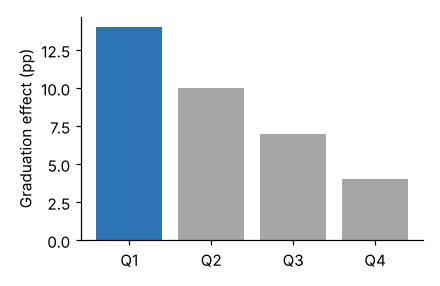
\includegraphics[width=0.7\textwidth]{fig_graduation.png}
\caption{Effect of tutoring on on-time graduation, by baseline math quartile.}
\label{fig:grad}
\end{figure}

\subsection{Test scores}
Scores rise by 0.28 SD after one year and remain 0.23 SD higher in grade 12, so fade-out is under 20\%
of the initial gain (Figure~\ref{fig:scores}).

\begin{figure}[h]
\centering
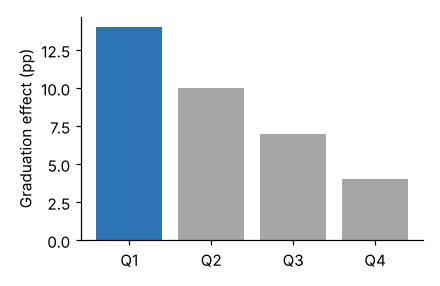
\includegraphics[width=0.7\textwidth]{fig_graduation.png}
\caption{Math scores by grade for tutored and control students.}
\label{fig:scores}
\end{figure}

\section{Mechanisms}
Holding grade 8 scores fixed reduces the graduation effect from 9 points to 1 point, which is not
significant. Holding credits earned fixed leaves it at 8 points.

\section{Conclusion}
One year of tutoring in grade 6 produces a graduation gain six years later, concentrated among
students who started behind. The main limitation is external validity: the study covers one urban district.

\bibliographystyle{plainnat}
\bibliography{refs}
\end{document}
